\chapter{Background}
\label{chapter:background}

This project aims to improve the efficiency of real-time rendering of 3D fractals. This chapter will focus on background theory for fractals, signed distance functions and sphere tracing. Afterwards, two possible methods of improving efficiency will be discussed, namely SDFs and temporal caching. Finally, some motivation for choosing these methods will be given.

\section{Rendering of Fractals}

\subsection{2D Fractals - The Mandelbrot Set}

\begin{figure}[ht]
	\centering
	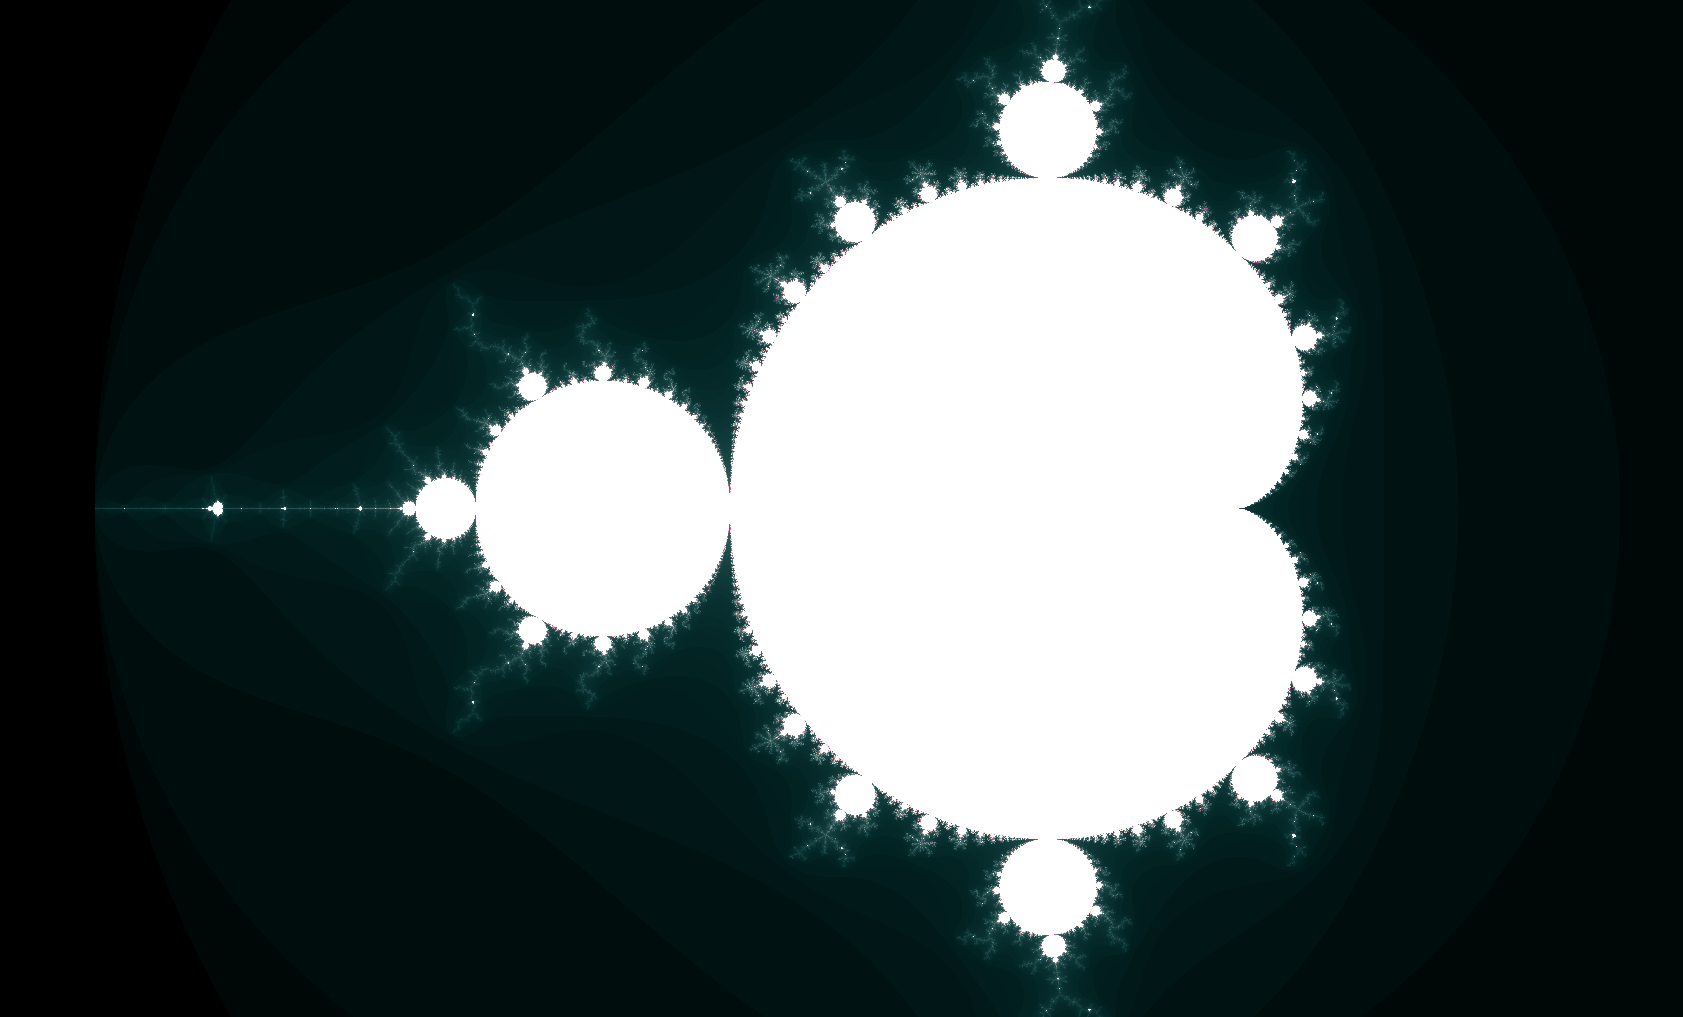
\includegraphics[width=0.65\linewidth, frame]{Images/Mandelbrot-2D-Full.png}
	\caption{The Mandelbrot set. The white points in the centre are inside the set.}
	\label{figure:mandelbrot-2d-full}
\end{figure}

The Mandelbrot set is the set of two-dimensional points that satisfy a certain constraint on the following complex quadratic equation:

\begin{equation} \label{equation:mandelbrot-2d}
	Z = {Z^2} + C
\end{equation}

where Z and C are complex numbers. The constraint on the points is that their orbit must be bounded. The value of Z is initialized to 0 and equation \ref{equation:mandelbrot-2d} is iterated over, each new value of Z being placed back in to the equation in the next iteration. If the length of the point Z does not exceed a threshold, then the point (represented by C) is in the Mandelbrot set \cite{devaney1999mandelbrot}.\newline

Figure \ref{figure:mandelbrot-2d-full} shows a generated Mandelbrot set. The real part of the point C is represented by the x-axis, and the imaginary part by the y-axis. Equation \ref{equation:mandelbrot-2d} is iterated over a maximum of five hundred times, and the threshold value is two. The pixels are coloured according to how many iterations are achieved before the length of Z exceeds the threshold.

\begin{figure} [ht]
	\centering
	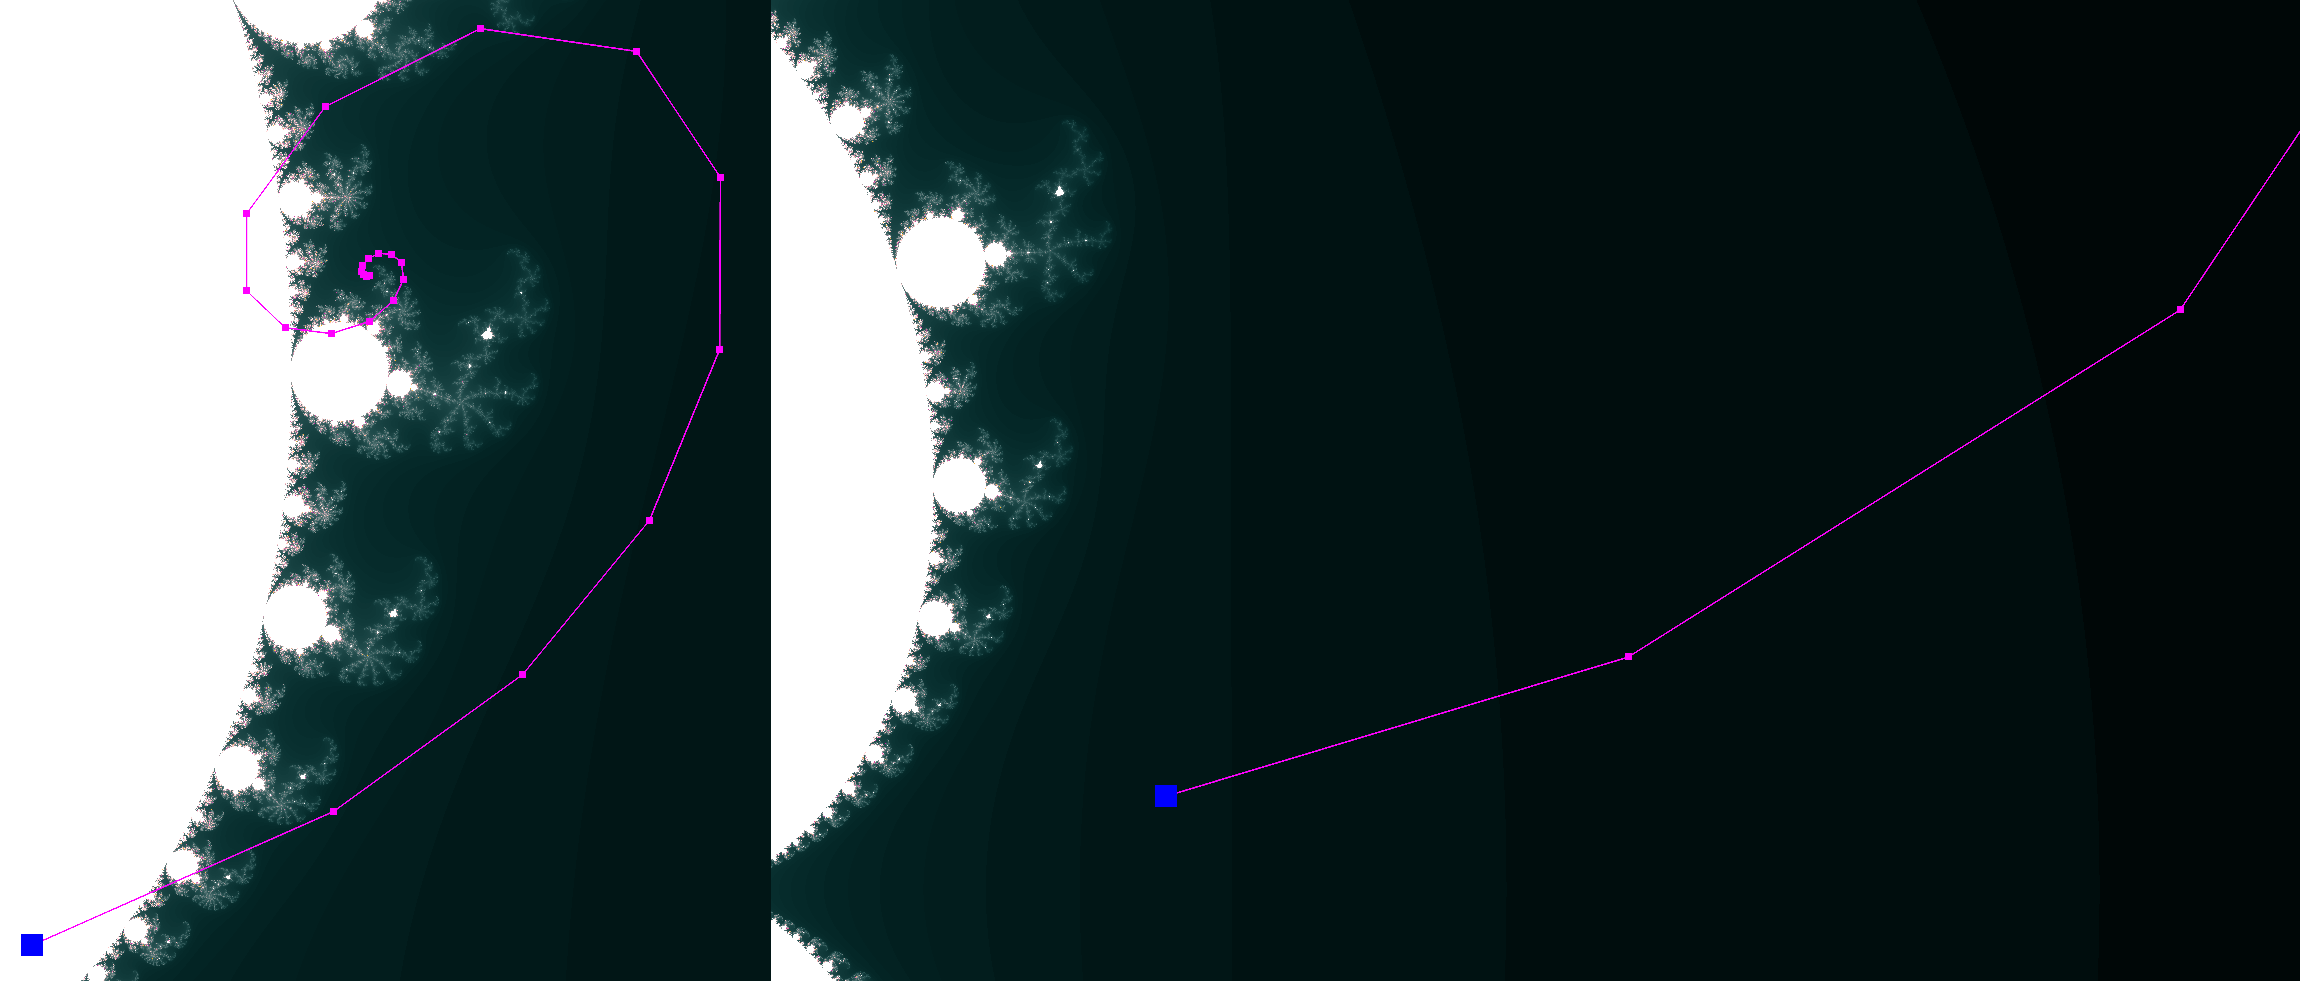
\includegraphics[width=0.8\linewidth, frame]{Images/Mandelbrot-2D-Iterations.png}
	\caption{Visualization of the first twenty five iterations of equation \ref{equation:mandelbrot-2d} on the initial points [0.3, 0.05] (left) and [0.5, 0.04] (right). The initial points are shown in blue.}
	\label{figure:mandelbrot-2d-iterations}
\end{figure}

\begin{figure} [ht]
	\centering
	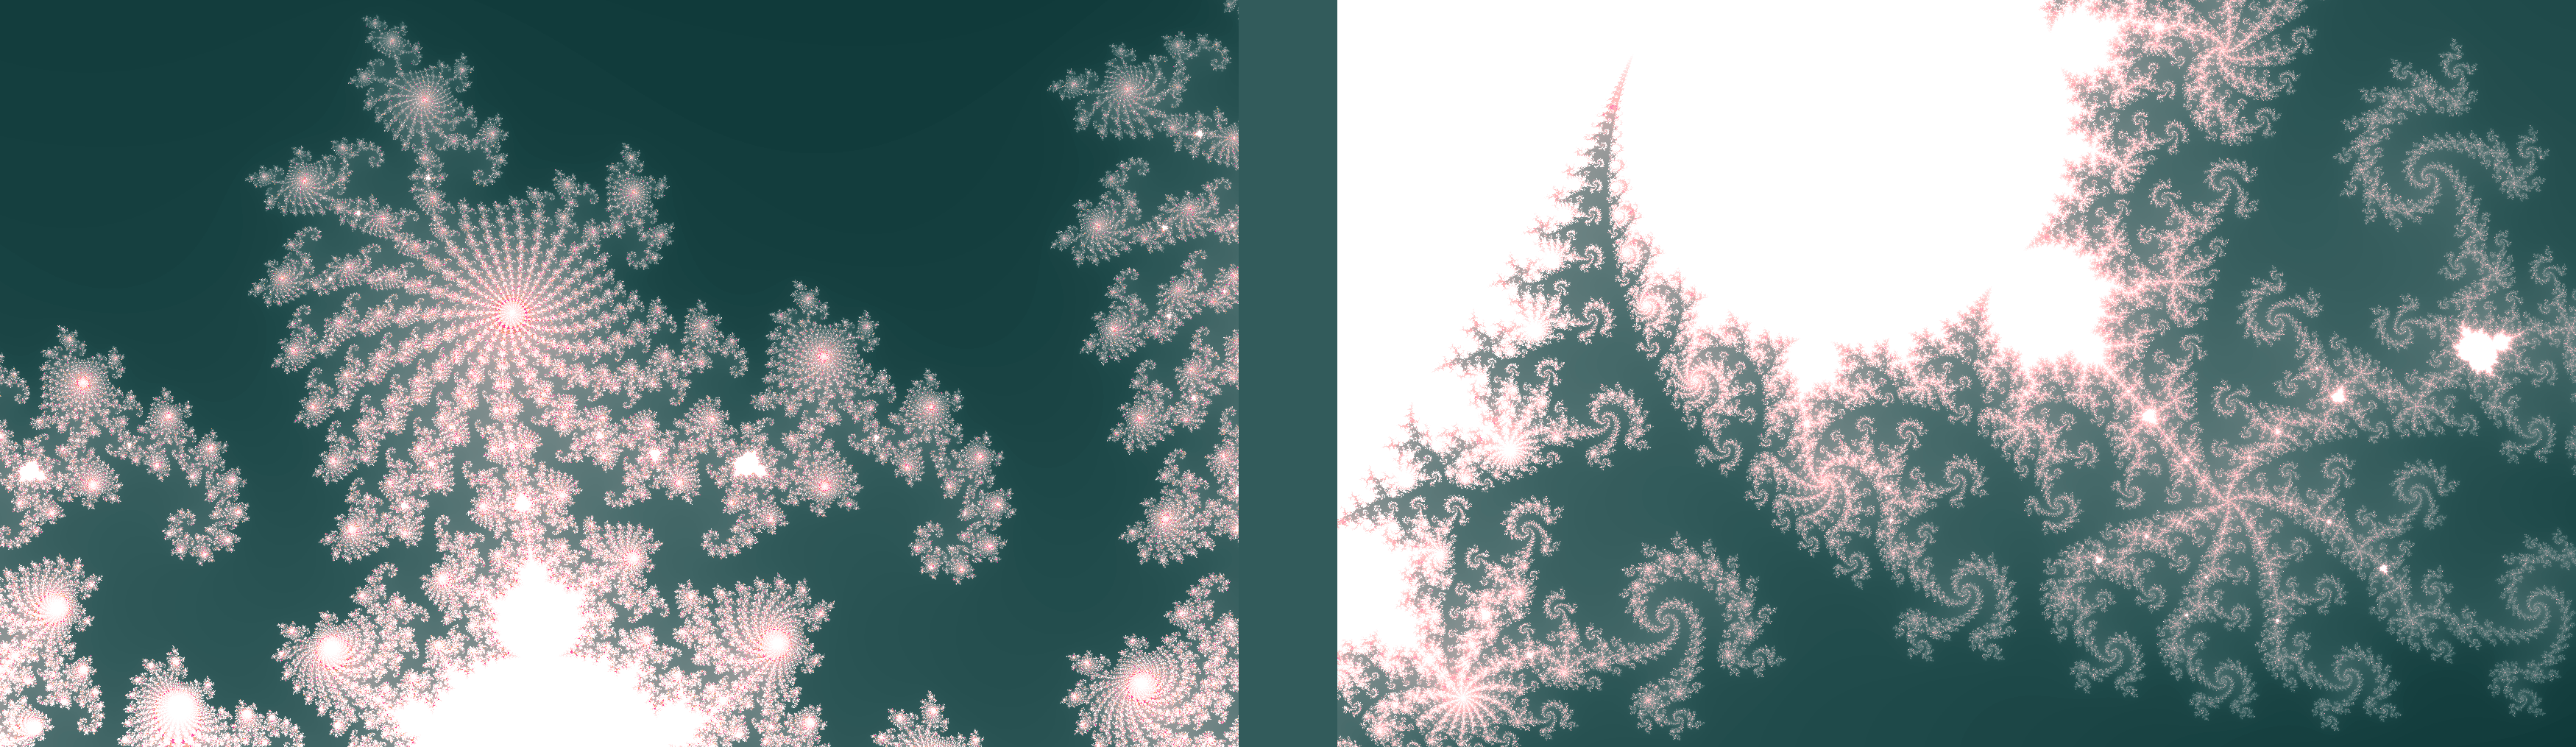
\includegraphics[width=0.8\linewidth, frame]{Images/Mandelbrot-2D-Zoom.png}
	\caption{Two different views of the Mandelbrot set, zoomed in.}
	\label{figure:mandelbrot-2d-zoom}
\end{figure}

Figure \ref{figure:mandelbrot-2d-iterations} illustrates the first twenty five iterations on two different points. For the first point, the iterations converge in a spiral shape and the length of Z never exceeds the threshold of two, therefore the point is in the Mandelbrot set and is coloured white. For the second point, the iterations diverge and exceed the threshold of two within a few iterations, so this point is not in the Mandelbrot set and is coloured dark.\newline

Figure \ref{figure:mandelbrot-2d-zoom} shows two zoomed-in views at the edge of the original shape. New patterns can be seen, as well as repeated ones, and even new instances of the original shape. This is because the Mandelbrot set has infinite detail, so if one decreases the range of the axes, new patterns will emerge \cite{ashlock2006evolutionary}.\newline

This project makes use of three-dimensional fractal rendering, so the next section will look at the challenge of bringing this infinite level of detail to three dimensions.

\subsection{3D Fractals - The Mandelbulb}

\begin{figure} [ht]
	\centering
	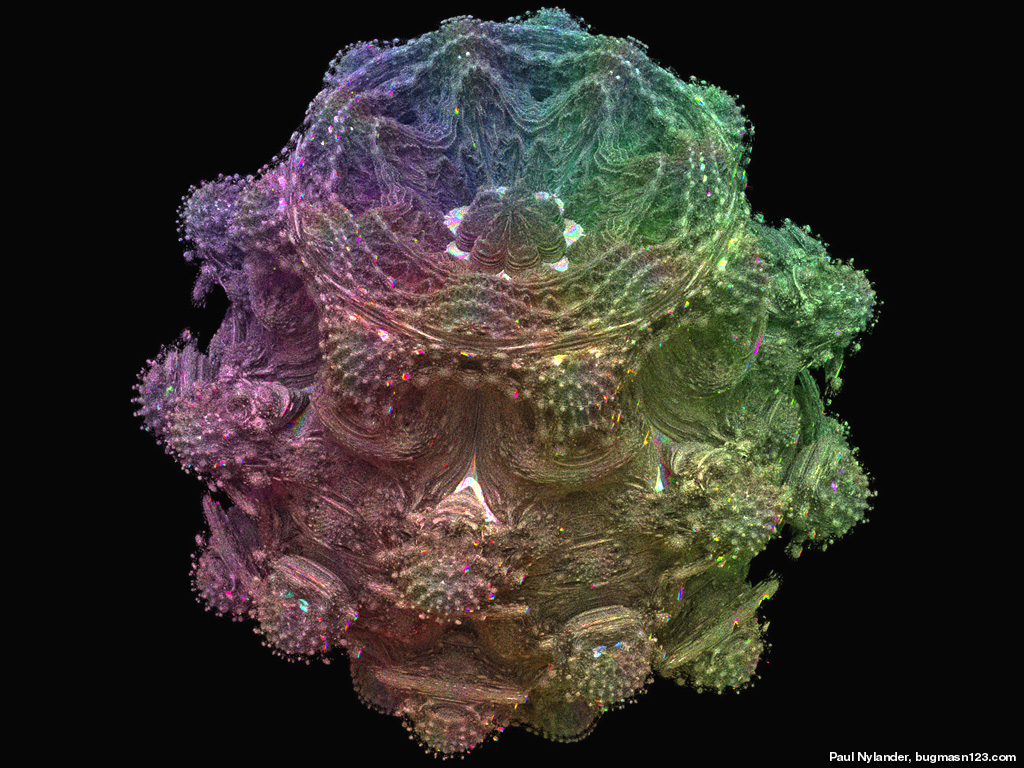
\includegraphics[width=0.5\linewidth, frame]{Images/Mandelbulb-First-Look.jpg}
	\caption{First look at the Mandelbulb, from Paul Nylander's website \cite{nylander-mandelbulb-image}.}
	\label{figure:mandelbulb-first-look}
\end{figure}

Since the Mandelbrot set is in two dimensions, and since complex numbers have only two components (real and imaginary), obtaining a true three-dimensional Mandelbrot set is a challenging task, and a mathematically rigorous three-dimensional Mandelbrot has not yet been found \cite{aron2009mandelbulb}.\newline

One attempt that seems to have come close was originated by Rudy Rucker in 1987. Rucker thought that expressing the three-dimensional points in spherical coordinates would allow the manipulation of the points in a similar way to the complex-number operations performed on the points in the two-dimensional Mandelbrot set \cite{rucker2009search}.\newline

Rucker did not have the computational power to accomplish a rendering of this idea, so it was put aside for twenty years, until Daniel White independently published a formula in 2007, which took the approach proposed by Rucker. White decided to approach the problem by considering the geometrical consequences of multiplying numbers in the complex plane, which amounts to rotating them \cite{aron2009mandelbulb}.\newline

White's formula produced images that looked promising, but they didn't have the level of detail that was expected from a true three-dimensional equivalent of the Mandelbrot set. A mathematician, Paul Nylander, raised White's formula to a higher power (eight), which would be equivalent to increasing the number of rotations of the point. The resulting image is shown in figure \ref{figure:mandelbulb-first-look}. The shape maintains excellent detail, even at high levels of magnification \cite {aron2009mandelbulb}.

The new shape, known as the Mandelbulb, has roughly the same formula as the Mandelbrot set (equation \ref{equation:mandelbrot-2d}):

\begin{equation} \label{equation:mandelbulb}
	Z = {Z^k} + C
\end{equation}

where Z is raised to an arbitrary power like so:

\begin{equation} \label{equation:mandelbulb-power}
	{Z^k} = {r^k}(sin[k\theta]cos[k\phi], sin[k\theta]sin[k\phi], cos[k\theta]).
\end{equation}

The variable r is the norm of Z (|Z|), $\theta$ is equal to arctan($Z_y$/$Z_x$) and $\phi$ is equal to |($Z_x$, $Z_y$)|/$Z_z$. The spherical coordinates of the point Z/|Z| are represented by $\theta$ and $\phi$. Equations \ref{equation:mandelbulb} and \ref{equation:mandelbulb-power} are sourced from Chapter 33 of the book Ray Tracing Gems II \cite{marrs2021ray}.

\subsection{Signed Distance Functions}

Signed distance functions provide an estimate of how close a point is to the surface of a shape. If the result of the function is positive, then the point is outside the surface. If the result is negative, then the point is inside the surface. If the result is zero, then of course the point is exactly on the surface of the shape described by the function \cite{roblesprocedural}.\newline

A signed distance function can be derived using the B\"{o}ttcher map for the fractal formula, which is a deformation of the space. Closer to the surface of the fractal, the space is deformed to a greater degree than parts further away from the surface, as shown in figure \ref{figure:julia-bottcher-map}. The deformations of the space occur in such a way as to map the exterior of the fractal to the exterior of a unit disk \cite{quilez-distance}.\newline

A rigorous mathematical explanation of the B\"{o}ttcher map will not be given in this paper, but a brief introduction is helpful to understand the derivation of the distance function for the Mandelbulb. The map can be calculated as follows:

\begin{equation} \label{equation:bottcher-map}
	{\phi_C[Z]} = {lim_{n\rightarrow\infty}[f^n[Z]]^{k^{-n}}}
\end{equation}

where the value of f[Z] is the same as in equation \ref{equation:mandelbulb} and n refers to the current iteration of the equation \cite{marrs2021ray}.\newline

Looking at equation \ref{equation:bottcher-map}, take a point Z that is not in the fractal, so that the function f$^n$[Z] grows as the number of iterations increases, tending towards infinity. For a large enough value of n, the term f$_n$[Z] will become vastly larger than the value of C (as the point is far from the fractal), meaning that C can reasonably be discarded \cite{marrs2021ray}.

\begin{figure} [ht]
	\centering
	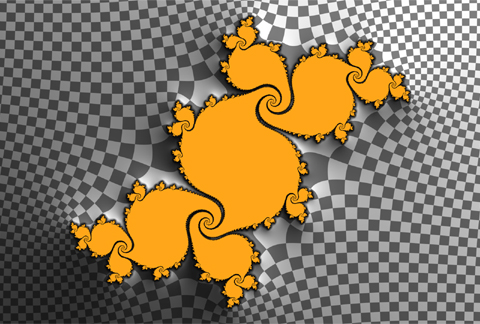
\includegraphics[width=0.5\linewidth, frame]{Images/Quilez-Bottcher-Map.jpg}
	\caption{The B\"{o}ttcher map generated for the Julia set (another two-dimensional complex fractal related to the Mandelbrot set), from the website of Inigo Quilez \cite{quilez-distance}.}
	\label{figure:julia-bottcher-map}
\end{figure}

From this casting away of C we obtain:

\begin{equation} \label{equation:mandelbulb-without-c}
	{f^{n+1}[Z] \approx {(f^n[Z])^k}}
\end{equation}

for points that are sufficiently far away from the surface of the fractal. Since the point at iteration n is far from the fractal, if one were to undo all of the iterations to get back to the original point at f$_0$[Z], we would obtain this expression:

\begin{equation} \label{equation:reverse-iterations}
	{{f_0^{n}[Z]}^{k^{-n}}} = Z
\end{equation}

and by extension, returning to the B\"{o}ttcher map:

\begin{equation} \label{equation:reverse-iterations-bottcher}
	\phi_0[Z] = Z
\end{equation}

which is the approximate result that equation \ref{equation:bottcher-map} gives when the function f$^n$[Z] ultimately diverges \cite{marrs2021ray}.\newline

Next, we will use something called the Hubbard-Douady potential, equal to the logarithm of the modulo of the B\"{o}ttcher map. This is a map of points onto a unit disk. Recall that the B\"{o}ttcher map maps the exterior of the fractal to the exterior of a unit disk. This now becomes important, as it enables us to use the Hubbard-Douady potential for all of our complex fractals. We now have a function that tends towards zero as the points approach the boundary of the fractal \cite{quilez-distance}:

\begin{equation} \label{equation:hubbard-douady}
	G[Z] = {lim_{n\rightarrow\infty}}\frac{log|{f^n}[Z]|}{k^n}.
\end{equation}

Equation \ref{equation:hubbard-douady} is not ready to be used as a distance measurement yet. However, it's possible to make it so. More detail is given in Ray Tracing Gems II, but a brief explanation will be given here. If we divide G[Z] by its gradient (obtaining this from the first-order Taylor expansion of the function), then we obtain an upper bound on the distance to the surface, which is desirable. The final equation for distance estimation therefore is \cite{marrs2021ray}:

\begin{equation} \label{equation:final-distance-estimate}
	d(Z) = {lim_{n\rightarrow\infty}}\frac{|f^n(Z)|log|f^n(Z)|}{|(f^n)'(Z)|}.
\end{equation}

\subsection{Ray and Sphere Tracing}

Ray tracing is a technique used for rendering scenes. Generally, a ray is a line that is cast from the camera or eye through each pixel of an image. Tests are performed to see which object (if any) is encountered by the ray first. By bouncing the ray from object to object, the program can gather the various light contributions from objects that reflect, emit or refract light \cite{haines2019ray}.\newline

Distance estimators can be used for ray tracing. If the approximate distance to the nearest surface can be calculated then the current point can be moved along the ray safely, until it is close enough to the surface to stop, according to this formula:

\begin{equation} \label{equation:sphere-tracing}
	{P_{n+1}} = {P_n} + \textbf{v}d({P_n})
\end{equation}

where P$_{n+1}$ is the point at the next step, P$_n$ is the point at the current step, \textbf{v} is the unit vector representing the ray direction and d(P$_n$) is the distance function acting on the current point \cite{marrs2021ray}.\newline

Using a distance function in this way is known as sphere tracing. The magnitude of the result of the distance function can be considered as the radius of a sphere. This sphere is guaranteed not to go through any part of the surface, making it safe to step according to the distance function result in any direction. For this guarantee to hold, the distance function must either be an exact calculation of the distance, or an underestimate \cite{hart1996sphere}.\newline

See figure \ref{figure:sphere-tracing}. This shows three scenarios for tracing a ray with the sphere tracing technique. At the bottom, the distance function is an exact measure of the distance to the nearest point on the surface. This is the ideal scenario, for correctness and performance. The top left image shows the result of a distance function which underestimates the distance each time. As a result, significantly more steps are taken along the ray, which will result in decreased performance. Lastly, the top right image shows the result of overestimating the distance. The ray ends up stepping past the boundary of the shape.

\begin{figure} [ht]
	\centering
	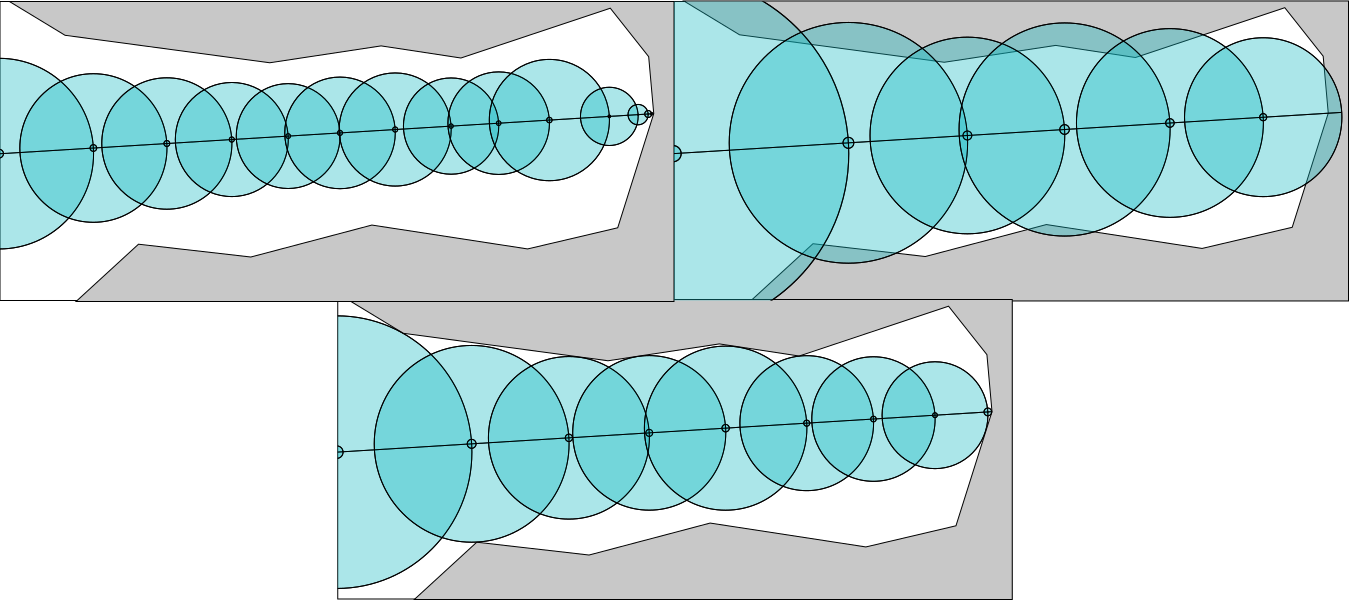
\includegraphics[width=0.65\linewidth, frame]{Images/Sphere-Tracing.png}
	\caption{Three scenarios in sphere tracing. Top left: Distance function underestimates distance, resulting in a loss of performance. Top right: Distance function overestimates distance, resulting in a loss of accuracy. Bottom: Distance function is exact.}
	\label{figure:sphere-tracing}
\end{figure}

\section{Optimization Methods}

\subsection{Signed Distance Fields}

A signed distance field is the result of discretizing a signed distance function over a finite space. The aim of the signed distance field is to reduce the need for evaluating potentially expensive signed distance functions for use in, for example, collision detection or ray tracing. Samples of the distance are taken at each point of the field (for example, at every voxel in a three-dimensional grid, as the case will be in this project) and stored for later use. Often, these samples are taken at the vertices of the grid, and when they are read, they are interpolated to get an approximation of the value at the specific point in the voxel \cite{koschier2016hierarchical}.\newline

Memory usage is a concern when using a signed distance field, especially if the shape requires high accuracy, as it will require a greater concentration of samples, especially near the surface. Some methods try to deal with this by increasing the amount of subdivision close to the surface or in areas with more complex geometry, and reducing it elswhere \cite{frisken2000adaptively}.

A common representation scheme for signed distance fields, and the one chosen for this project, is an eight-dimensional binary tree, also known as an octree. The nodes of the tree represent areas of the space, and at each level of the tree, these areas get exponentially smaller. Leaf nodes contain the information necessary for construction of the scene. Other nodes point to eight child nodes each, so that leaf nodes can be reached by searching the tree, starting with the root \cite{meagher1982geometric}.\newline

This structure, being constructed out of cubes, is simple to manipulate and search. All of the nodes of the tree can be kept in a specific order, which makes indexing very simple, since the tree can just be traversed in a specific order, rather than searching the space itself for the correct cube \cite{meagher1982geometric}.

\subsection{Temporal Caching} \label{section:temporal-caching}

Temporal caching methods rely on the idea that the contents of an image don't change much from frame to frame; they are temporally coherent. With this in mind, a possible performance booster can be implemented for ray tracing, which uses information (such as colours, lighting data or positions) from previous states to speed up or provide a hint for calculations in the current frame \cite{cosenza2008estimating}.\newline

Taking advantage of temporal coherence in ray tracing is of special interest in the case of global illumination data, which is very expensive to calculate. In order to maintain spatial coherence between frames, methods often perform temporal reprojection, which maps the location of the point on the surface from the current frame to the previous frame, so that it samples from similar areas in the scene \cite{scherzer2012temporal}.\newline

Consider the scenario in which a ray travels through a room, hitting the back wall. In the next frame, the camera has moved, and the same ray now intersects a closer object, say a chair. However, the sampled distance from the previous frame already places the point behind the chair, rendering the chair invisible. The method used in this project needs to take this problem into account, since the camera position and rotation will change.\newline

Determining whether a pixel value is invalid can be done in a few ways. For example, testing the angle between the normal of the previous frame and the current ray, and recasting the ray if the angle exceeds some threshold. It could also be done by comparing the depth of previous frames with the depth of the current frame, though this would likely work better for mesh geometry, as it requires knowing the exact depth in the current frame, the calculation of which this project is trying to avoid \cite{weier2016foveated}.

\section{Implementation of Optimization Methods}

\subsection{Signed Distance Field}

The use of an SDF is intended to provide a cheaper way of evaluating the distance at any point around the fractal shape than calculating the signed distance using the given function. If this is possible, then performance boosts will be expected when rendering the fractals in real time.\newline

The octree data structure has been chosen for this project for its simplicity, and for the ability to be selective about when to perform a memory read, which is expensive compared to calculations on the GPU. Memory usage will need to be considered, as a very high resolution representation of the space will be costly. For this project, very fine detail is not needed, so a relatively coarse field can be used. However, accuracy is still a concern. Chapter \ref{chapter:implementation} on implementation will discuss decisions made to tackle this problem.\newline

The octree representation chosen will not be sparse. This is because there is a need to reduce the frequency of memory reads as much as possible, and having a sparse structure would introduce the need to store additional information, used for traversing the tree. If the octree is not sparse, the required voxel index can be calculated, rather than read from memory.

\subsection{Temporal Cache}

\begin{figure} [ht]
	\centering
	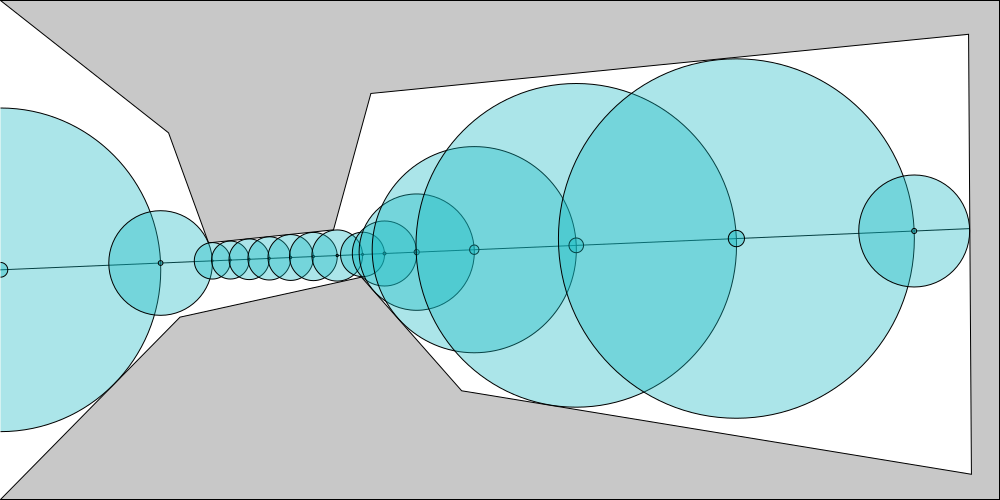
\includegraphics[width=0.65\linewidth, frame]{Images/Sphere-Tracing-Bottleneck.png}
	\caption{A particular scenario in sphere tracing, where the ray passes close to some geometry, but never intersects. This slows the ray down and results in a loss of performance.}
	\label{figure:sphere-tracing-bottleneck}
\end{figure}

The goal of using temporal caching for rendering three-dimensional fractals is to reduce the number of iterations required to get to the surface. This is a different approach than using a signed distance field, which is intended to reduce the cost of the iterations.\newline

The information required to render the scenes in this project is the distance travelled by each ray. For a still image (no camera movement), the result of the last frame can be sampled and used again exactly the same in the next frame, skipping all sphere tracing iterations. Of course for real time rendering, an image is likely to change, either because of moving geometry, or camera changes. To tackle this, a test will be performed to see if the camera has moved too much, and a effort will be made to have a consistent, but preferably small, underestimate of the true distance, so that the rays don't overshoot. difference between them exceeds some threshold, then the ray will be recast. I chose not to use the angle between the normal and current ray because that would require storage of the normal, and therefore more sampling from the cache every frame.\newline

One scenario of interest in this project is illustrated in figure \ref{figure:sphere-tracing-bottleneck}. The ray passes very close to the surface of the shape along its path, but never intersects that part of the shape. This results in smaller steps for the sphere tracing algorithm, and a loss of performance, as a significant number of iterations are expended getting past the bottleneck in the scene. This paper proposes that a temporal caching method could be employed that provides a significant performance boost by bypassing the bottlenecks in these scenarios.